\chapter{Order and transfers}
\label{ch:order}

After the decomposition of Chapter~\ref{ch:split} the mower has a list of
cells to mow, each by its own passes. Two questions are left: in which
order to mow the cells, and how to drive from one to the next, around the
holes and without leaving the lawn. This chapter answers both, and puts
together the complete planner, whose results end the chapter.

\section{Four ways to mow a cell}

The passes of a cell, in the order of Chapter~\ref{ch:swaths}, can be driven
from the first to the last or from the last to the first, and the first
pass can be driven in either direction; every later pass is driven the
other way from the one before.

\begin{definition}{Way}{way}
  A \emph{way} of mowing a cell is a choice of the direction of its order
  of passes (forwards or backwards) and of the direction of its first pass.
  Each way has an \emph{entry}, the pose of the rear axle at the start of
  its first pass, and an \emph{exit}, the pose at the end of its last pass.
\end{definition}

The four ways take the same time inside the cell (the same passes and the
same turns, in mirror image), but their entries and exits differ: two
corners of the cell for the entries, two for the exits. A transfer joins
the exit of one cell to the entry of the next.

\section{The order as a travelling salesman problem}

\begin{definition}{Order of the cells}{cellorder}
  For $n$ cells with $k$ ways each, an \emph{order} is a sequence of $n$
  pairs $(i_1, a_1), \dots, (i_n, a_n)$ where $i_1, \dots, i_n$ is a
  permutation of the cells and $a_j$ the way cell $i_j$ is mowed. With
  $T(p, q)$ the time of a transfer from the pose $p$ to the pose $q$, and
  $q_0$ the pose at the end of the headland, its cost is
  \[
    C = T\bigl(q_0, \mathrm{entry}(i_1, a_1)\bigr)
      + \sum_{j=1}^{n-1} T\bigl(\mathrm{exit}(i_j, a_j),
        \mathrm{entry}(i_{j+1}, a_{j+1})\bigr).
  \]
\end{definition}

This is a \emph{generalised} travelling salesman problem: every cell is a
group of $k$ ``cities'' (its ways), and the tour must visit one city per
group. With a handful of cells, it can be solved exactly by dynamic
programming over the subsets of cells, the method of Held and
Karp~\cite{held1962dynamic}.

\begin{proposition}{Dynamic programming over subsets}{heldkarp}
  Let $D(S, i, a)$ be the least cost of an order that mows exactly the
  cells of the set $S$ and ends with cell $i \in S$ mowed in the way $a$.
  Then
  \begin{align*}
    D(\{i\}, i, a) &= T\bigl(q_0, \mathrm{entry}(i, a)\bigr), \\
    D(S \cup \{j\}, j, b) &= \min_{i \in S,\, a}
      \Bigl[ D(S, i, a) + T\bigl(\mathrm{exit}(i, a),
      \mathrm{entry}(j, b)\bigr) \Bigr]
  \end{align*}
  for $j \notin S$, and the best order costs $\min_{i, a} D(\{1, \dots,
  n\}, i, a)$. Computing all the values takes $O(2^n n^2 k^2)$ operations.
\end{proposition}

\begin{proof}
  An order that mows the cells of $S \cup \{j\}$ and ends with $(j, b)$
  is an order of the cells of $S$, ending with some $(i, a)$, followed by
  the transfer to $(j, b)$; its cost is the cost of the first part plus that
  of the transfer. The best one therefore uses a best order of $S$ ending
  with $(i, a)$, for the best choice of $(i, a)$. There are $2^n$ sets, $n
  k$ ends and $n k$ next steps for each, hence the count.
\end{proof}

\begin{example}{The garden}{gardendp}
  With $n = 4$ cells and $k = 4$ ways, the table has at most $2^4 \times 4
  \times 4 = 256$ entries and the recursion makes $2^4 \times (4 \times
  4)^2 = 4096$ steps. It needs the times of $4 \times 4 = 16$ transfers
  from the headland and $4 \times 3 \times 4^2 = 192$ between cells. Up to
  about ten cells the computation stays below a second; beyond, a greedy
  order improved by local moves, as for the passes in
  Chapter~\ref{ch:swaths}, would replace it.
\end{example}

\section{The time of a transfer}

Solving the problem needs $T(p, q)$ for every pair of ways, before any path
is planned. The planner first tries the fastest Reeds--Shepp path from $p$
to $q$ that the collision checker accepts (Chapter~\ref{ch:headlands}): if
there is one, its time is $T(p, q)$. Otherwise it estimates $T(p, q)$ by
the larger of two times, each one too short:

\begin{description}
  \item[The free time.]
    \leavevmode\\
    The time of the fastest Reeds--Shepp path, which ignores the holes and
    the border.
  \item[The grid time.]
    \leavevmode\\
    The length of the shortest path from $p$ to $q$ on a grid of
    \SI{25}{\centi\metre} cells over the lawn, at the mowing speed: it goes
    around the holes but turns on the spot.
\end{description}

The grid distance is computed once for every goal $q$, by Dijkstra's
algorithm from $q$ over the cells that the mower's reference point can
occupy, with steps to the eight neighbours of a cell. Only then are the
transfers of the chosen order planned, with the search of the next section
where no direct path exists.

\section{Hybrid A*}
\label{sec:hybrid}

The planner has used a search for paths around obstacles since
Chapter~\ref{ch:headlands}: \emph{Hybrid A*}, introduced by Dolgov, Thrun,
Montemerlo and Diebel~\cite{dolgov2010path} for autonomous cars in car parks.
It is the A* search on a graph whose nodes are poses reached by driving,
with two twists.

\begin{description}
  \item[Moves.]
    \leavevmode\\
    From a pose, the mower drives \SI{0.6}{\metre} forward or in reverse
    on one of five arcs, of curvature $-\kmax$, $-\kmax/2$, $0$, $\kmax/2$
    and $\kmax$: ten moves, each checked for collision. A move costs its
    driving time (at the speed of Chapter~\ref{ch:measuring} for its kind),
    plus $t_{\mathrm{shift}} = \SI{2}{\second}$ if it changes the direction
    of travel.
  \item[Cells.]
    \leavevmode\\
    The poses reached are exact, not rounded to a grid, but only the best
    one is kept in each cell of a grid over $(x, y, \theta)$ of
    \SI{0.3}{\metre} by \SI{0.3}{\metre} by $5°$: a pose that reaches a
    cell already reached at a lower cost is dropped. This keeps the search
    finite.
\end{description}

A* expands first the pose with the smallest $g + h$, where $g$ is the cost
from the start and $h$ an estimate of the cost to the goal. The planner
uses
\[
  h(p) = \frac{\max\bigl(\ell_{\mathrm{RS}}(p, q),\;
    \ell_{\mathrm{grid}}(p, q)\bigr)}{v_{\max}},
\]
where $\ell_{\mathrm{RS}}$ is the length of the shortest Reeds--Shepp path
from $p$ to the goal $q$, $\ell_{\mathrm{grid}}$ the grid distance of the
previous section, and $v_{\max} = \SI{1.2}{\metre\per\second}$ the highest
speed.

\begin{proposition}{The heuristic is nearly a lower bound}{heuristic}
  Every collision-free path from $p$ to $q$ takes at least
  $\ell_{\mathrm{RS}}(p, q)/v_{\max}$, and at least
  $\ell_{\mathrm{grid}}(p, q)/(1.083\, v_{\max})$ up to the size of a grid
  cell.
\end{proposition}

\begin{proof}
  A path that the mower can drive is a path of curvature at most $\kmax$,
  forward or in reverse, so it is at least as long as the shortest such
  path ignoring obstacles, the Reeds--Shepp path (Chapter~\ref{ch:paths});
  driving a length $\ell$ takes at least $\ell / v_{\max}$. The point $P$
  stays in free cells of the grid, and a path on an 8-connected grid is at
  most $1/\cos(22.5°) = 1.083$ times longer than the straight segments it
  follows (the worst case is a direction halfway between a side and a
  diagonal step); so the grid distance overestimates the length of any
  path through the same cells by at most this factor, plus the rounding of
  the end points to their cells.
\end{proof}

A heuristic that never overestimates makes A* return an optimal path. This
one may overestimate a little, and the cells drop poses that a finer
search would have kept, so Hybrid A* gives a good path rather than the
best one; it is also not guaranteed to find one, within its budget of 6000
expansions, when one exists. Its second twist makes it fast in open
spaces: every ten expansions it tries to finish with a direct
collision-free Reeds--Shepp path to the goal, which succeeds as soon as the
goal is in sight (Figure~\ref{fig:hybrid}).

\begin{figure}[ht]
  \centering
  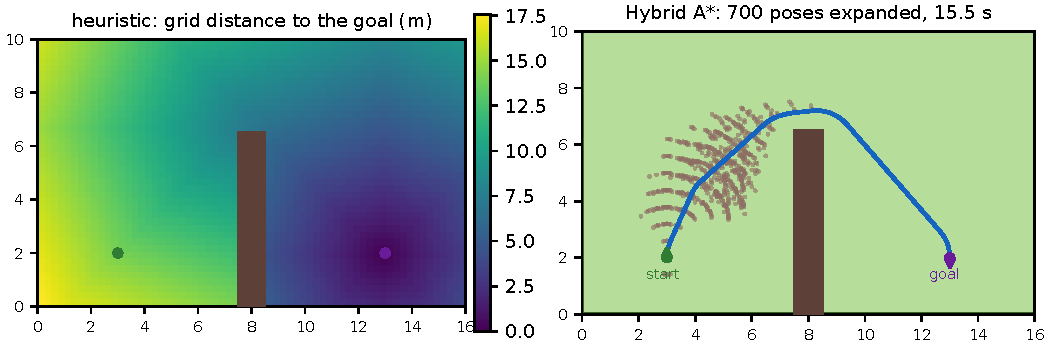
\includegraphics[width=\textwidth]{figures/hybrid}
  \caption{Hybrid A* on a \SI{16}{\metre} by \SI{10}{\metre} lawn with a
    wall (brown), from the green pose (heading north) to the purple one
    (heading south). Left: the grid distance to the goal, the part of the
    heuristic that knows about the wall. Right: the poses expanded (brown
    dots), fanning out along the arcs, and the path found (blue): the
    search reaches the top of the wall, from where a direct Reeds--Shepp
    path to the goal is free.}
  \label{fig:hybrid}
\end{figure}

\section{The complete planner}

\begin{enumerate}
  \item Choose the order of the passes: \code{adjacent} or \code{skip}
    (Chapter~\ref{ch:swaths}). The rest is done for both, and the faster
    plan is kept.
  \item Count the headland passes from the room the turns need
    (Proposition~\ref{prop:headlandcount}), plan them and join them
    (Chapter~\ref{ch:headlands}).
  \item Cut the interior into cells, each with its direction
    (Chapter~\ref{ch:split}).
  \item List the four ways of each cell, estimate the transfers, and
    choose the order of the cells and their ways
    (Proposition~\ref{prop:heldkarp}).
  \item Plan the passes of each cell in the chosen way, the turns between
    them, and the transfer to its entry (direct, or by Hybrid A*).
\end{enumerate}

\begin{figure}[p]
  \centering
  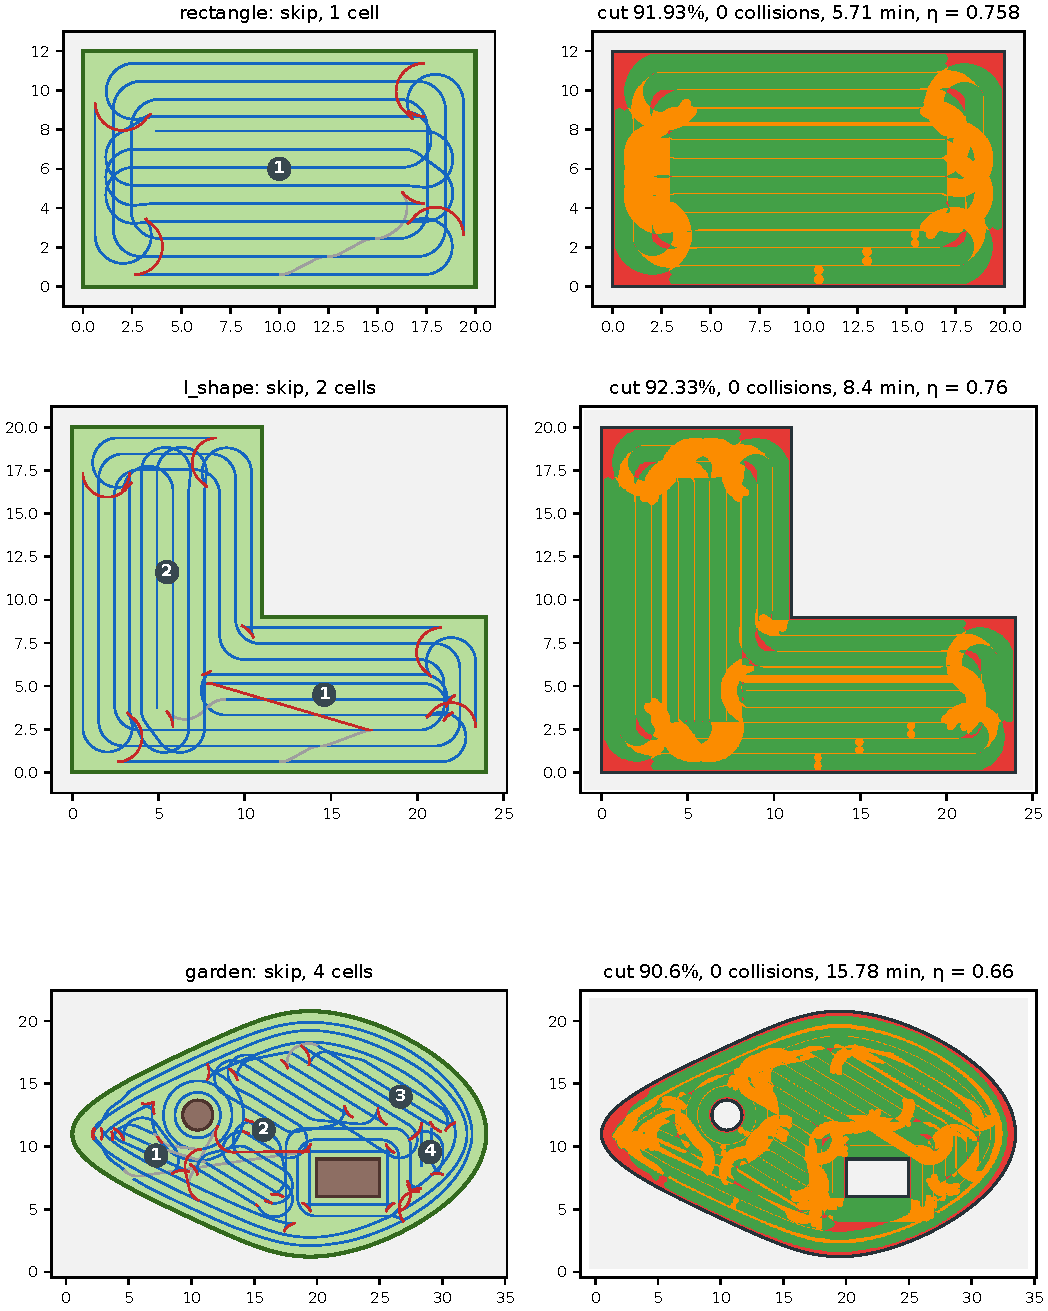
\includegraphics[width=\textwidth]{figures/final}
  \caption{The complete planner on the three example lawns. Left: the path
    of the rear axle (blue forward, red reverse, grey blades off) and the
    order of the cells (numbers). Right: the grass cut (green once, orange
    twice, red missed), with the efficiency $\eta$ of
    Definition~\ref{def:efficiency}. The order of the passes with jumps
    (\code{skip}) was the faster on all three lawns.}
  \label{fig:final}
\end{figure}

\begin{center}
\begin{tabular}{@{}lrrrrrr@{}}
  \toprule
  lawn & cells & cut & collisions & time & lower bound & $\eta$ \\
  \midrule
  rectangle & 1 & 91.9\% & 0 & \SI{5.71}{\minute} & \SI{3.31}{\minute}
    & 0.758 \\
  L-shape & 2 & 92.3\% & 0 & \SI{8.40}{\minute} & \SI{4.64}{\minute}
    & 0.760 \\
  garden & 4 & 90.6\% & 0 & \SI{15.78}{\minute} & \SI{5.90}{\minute}
    & 0.660 \\
  \bottomrule
\end{tabular}
\end{center}

The lower bound is the time to drive the bound $\ell_{\mathrm{mow}}$ of
Theorem~\ref{thm:lowerbound} at mowing speed, with no turn.
Figure~\ref{fig:breakdown} shows where the time goes. The order of the
cells changes little: on the garden with the lateral order of the passes,
the optimal order saves \SI{0.16}{\minute} over the greedy one of
Chapter~\ref{ch:split} (\SI{15.96}{\minute} against \SI{16.12}{\minute}),
and with the order with jumps both find the same order. On the L-shape the
optimal order is estimated \SI{4.7}{\second} faster but comes out
\SI{1}{\second} slower, within the error of the estimates. The transfers,
blades off, are only 12 to \SI{14}{\percent} of the time. Most of the time
beyond the lower bound is spent in arcs, in reverse and stopping to change
direction: on the garden, whose curved border makes the headland rings
arcs and whose oblique cells make the turns long, these take
\SI{10.6}{\minute} out of \SI{15.8}{\minute}.

\begin{figure}[ht]
  \centering
  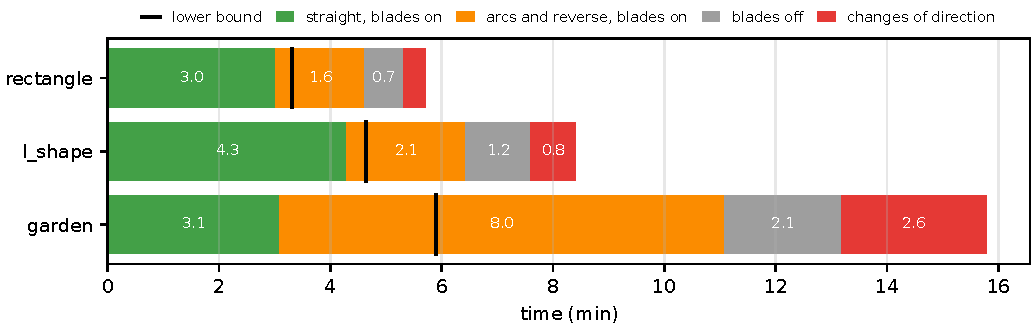
\includegraphics[width=\textwidth]{figures/breakdown}
  \caption{Where the time goes in the plans of Figure~\ref{fig:final}, in
    minutes: straight with the blades on (the passes and the straight parts
    of the headland), arcs and reverse with the blades on (turns, corners,
    the curved parts of the headland), transfers with the blades off, and
    the stops of \SI{2}{\second} at each change of direction. Black: the
    lower bound.}
  \label{fig:breakdown}
\end{figure}

\begin{inwords}
  The cells are mowed in the order that makes the transfers between them
  shortest, found exactly by trying all orders in a clever way; the
  transfers themselves are planned by a search that drives short arcs
  forward and in reverse, guided by an estimate of the remaining time.
  On these lawns the order hardly matters: the time is lost in turns,
  curves and stops, which the next chapters examine.
\end{inwords}

\begin{incode}
  \code{mowersim/planning/planner.py}: \code{cell\_ways}
  (Definition~\ref{def:way}), \code{TransferCost}, \code{order\_cells}
  (Proposition~\ref{prop:heldkarp}), \code{greedy\_order}, \code{plan} (the
  complete planner) and \code{time\_breakdown}.
  \code{mowersim/planning/search.py}: \code{grid\_distance} and
  \code{hybrid\_astar}. From the command line:
  \begin{verbatim}
python -m mowersim plan lawns/garden.json --png garden.png
  \end{verbatim}
\end{incode}
